% Drawing 43/04-15 -- folder 43, batch 04, archive page 68 (PDF page 69).
% Transcription: à gauche, des croquis : un court segment épais entre deux gros points, une graduation au milieu, souligné d'une petite accolade ; un long segment à deux graduations près du bout gauche ; au-dessous, deux points entourés d'un petit cercle, joints par deux chaînes (l'une au-dessus, passant par un gros point, l'autre au-dessous, à trois points), chacune enveloppée d'une accolade courbe ; à droite, une seconde figure de trois points avec des traits et des accolades ; en haut à droite, un point et un long trait terminé par un point.
% Kind: segments; two points joined by two chains under braces. Method 2 (schematic redraw from the facsimile). Status: partial.
% Notes: Ink. (1) Short heavy segment between two heavy dots with a middle tick and a small brace under its left half. (2) Long segment with a tick at the left end, a second tick close to it and a heavy end at the right. (3) Two ringed points; an upper chain from the left point through a heavy dot to the right point, with a curly brace over it; a lower chain with two small dots, and a curly brace under it ending at a dot near the right point. (4) Right: three dots on a line, a stroke rising from the first, a heavy stroke with a brace above between the second and third, a heavy brace and a stroke below. (5) Top right: a dot, then a long thin stroke ending in a dot. Still differs: the braces are freehand curves on the page and are drawn as simple arcs with a cusp; figure (4) runs off the right edge of the crop and is partly a reading. Redrawn 2026-11-12 (issue 128): to check again.
% Coordinates: 1 unit = 1 mm = 1/100 of the crop width, y downwards as on the crop (bbox in page fractions: [0.14, 0.49, 0.56, 0.67]).
% Redrawn by Claude (claude-fable-5-2), issue #128, 2026-11-12; not checked by a human; not compiled (no TeX in the session).
% Rights: reproduces part of the work -- behind RENDER_TRANSCRIPTS, never published by itself.
\documentclass[tikz,border=3pt]{standalone}
\usepackage{amsmath,amssymb}
\usetikzlibrary{patterns,arrows.meta}
\tikzset{pencil/.style={black!45}, struck/.style={black!35}, mpt/.style={circle,draw,inner sep=1.3pt}, pt/.style={circle,fill,inner sep=0.9pt}, opt/.style={circle,draw,fill=white,inner sep=1.1pt}, Rd/.style={red!75!black}, Gn/.style={green!45!black}, Br/.style={brown!70!black}}
\begin{document}
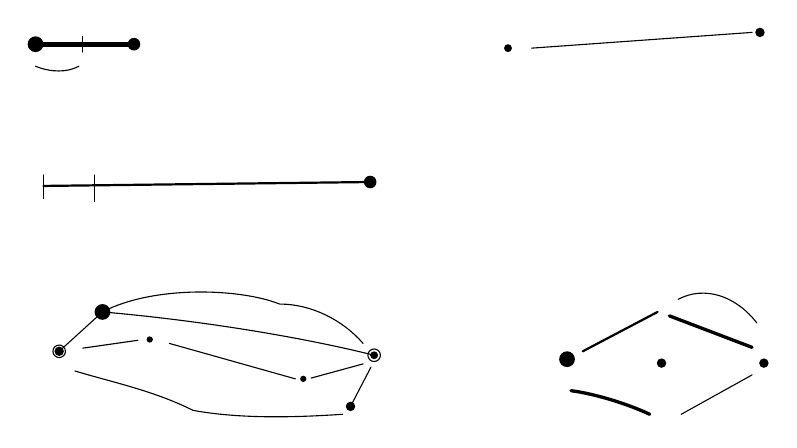
\begin{tikzpicture}[x=1mm,y=-1mm,line cap=round,line join=round,font=\small]
% (1)
\draw[line width=1.8pt] (7,7) -- (19.5,7);
\fill (7,7) circle [radius=1];
\fill (19.5,7) circle [radius=0.8];
\draw (13,6) -- (13,8);
\draw (7,9.8) .. controls (9,10.6) and (11,10.6) .. (12.5,9.8);
% (2)
\draw[thick] (8,25) -- (49.5,24.5);
\draw (8,23.6) -- (8,26.6);
\draw (14.5,23.6) -- (14.5,27);
\fill (49.5,24.5) circle [radius=0.8];
% (3)
\coordinate (A) at (10,46);
\coordinate (B) at (50,46.5);
\coordinate (C) at (15.5,41);
\node[opt,inner sep=1.6pt] at (A) {};
\node[opt,inner sep=1.6pt] at (B) {};
\fill (A) circle [radius=0.6];
\fill (B) circle [radius=0.5];
\fill (C) circle [radius=1];
\draw (A) -- (C);
\draw (C) .. controls (27,42) and (40,44) .. (B);
\draw (C) .. controls (22,37.6) and (33,38) .. (38,40) .. controls (42,40) and (46,42) .. (48.6,45);
\draw (13,45.6) -- (20,44.6);
\fill (21.5,44.5) circle [radius=0.4];
\draw (24,45) -- (40,49.5);
\fill (41,49.5) circle [radius=0.4];
\draw (42,49.4) -- (48.6,47.6);
\draw (12,48.5) .. controls (17,50) and (22,51) .. (27,53.5) .. controls (33,54.6) and (40,54.4) .. (46,54);
\draw (47,53) -- (49.6,48);
\fill (47,53) circle [radius=0.6];
% (4)
\fill (74.5,47) circle [radius=1];
\fill (86.5,47.5) circle [radius=0.6];
\fill (99.5,47.5) circle [radius=0.6];
\draw[thick] (76.5,46) -- (86,41);
\draw[very thick] (87.5,41.5) -- (98,45.5);
\draw (88.6,39.4) .. controls (92,37.6) and (96,39) .. (98.6,42.4);
\draw[very thick] (75,51) .. controls (78,51.4) and (82,52.6) .. (85,54);
\draw (89,54) -- (98,49);
% (5)
\fill (67,7.5) circle [radius=0.5];
\draw (70,7.5) -- (98,5.5);
\fill (99,5.5) circle [radius=0.6];
\end{tikzpicture}
\end{document}
